%! suppress = TooLargeSection
\documentclass[12pt,letterpaper,oneside,reqno]{amsart}
\usepackage{amsfonts}
\usepackage{amsmath}
\usepackage{amssymb}
\usepackage{amsthm}
\usepackage{float}
\usepackage[font=small,labelfont=bf]{caption}
\usepackage[left=1in,right=1in,bottom=1in,top=1in]{geometry}
\usepackage[pdfpagelabels,hyperindex,colorlinks=true,linkcolor=blue,urlcolor=magenta,citecolor=green]{hyperref}
\usepackage{graphicx}

\linespread{1.25}

%--------Meta Data: Fill in your info------
\title[RSA Encryption: Behind the scenes]{RSA Encryption: Behind the scenes}
\author[Petro Kolosov]{Petro Kolosov}
\keywords{Algorithms, Computer science, Cryptography, RSA, Number Theory}
\date{\today}
\hypersetup{
    pdftitle={RSA Encryption: Behind the scene},
    pdfsubject={Algorithms, Computer science, Cryptography, RSA, Number Theory},
    pdfauthor={Petro Kolosov},
    pdfkeywords={Algorithms, Computer science, Cryptography, RSA, Number Theory}
}
\begin{document}
    \begin{abstract}
        Simple explanation of the main idea behind the RSA encryption.
    \end{abstract}
    \maketitle
    \tableofcontents


%    \section{One way functions}\label{sec:one-way-functions}
%    One-way function -- is the function that is easy to compute on every input, but
%    hard to invert given the image of a random input.
%    For instance, the function
%    \begin{equation*}
%        f(m) = m^e \bmod N = C
%    \end{equation*}
%    where $e, N$ are public constants is one-awy function,
%    because it is easy to compute $C$ given $m$, however it is hard to compute $m$ given $C$.
%
%
%    \section{Euler's totient theorem}\label{sec:euler's-totient-theorem}
%    Given a positive composite integer $N$ and its prime factorization $p_1^{e_1}\cdot p_2^{e_2} \cdots p_k^{e_k}$,
%    then Euler's totient function $\phi(N)$ is defined as
%
%    \begin{equation}
%        \phi(N) = (p_1^{e_1} - p_1^{e_1 - 1}) \cdot (p_2^{e_2} - p_2^{e_2 - 1}) \cdots (p_k^{e_k} - p_k^{e_k - 1})
%        \label{eq:euler-totient-theorem}
%    \end{equation}
%
%    In particular, for the positive composite integer $N$ such that its factorization is $N = p_1 \cdot p_2$,
%    the Euler's totient function $\phi(N)$ is
%
%    \begin{equation}
%        \phi(N) = (p_1 -1) \cdot (p_2 - 1)\label{eq:euler-theorem-partial}
%    \end{equation}
%
%    Moreover, Euler's theorem relates the modular division and exponent.
%    Given a positive integer number $m$ we have
%    \begin{equation}
%        m^{\phi(N)} = 1 \bmod N\label{eq:euler-theorem-modular}
%    \end{equation}
%    It means that reminder of division $m^{\phi(N)}$ by $N$ is always 1.
%    Therefore, by the equality $1^K = 1$
%    \[
%        M^{K \cdot \phi(N)} = 1 \bmod N
%    \]
%    Now we are able to multiply both parts by $M$ so that we get
%    \[
%        M \cdot M^{K \cdot \phi(N)} = M^{K \cdot \phi(N) + 1} = M \bmod N
%    \]
%
%
%    %! suppress = TooLargeSection


    \section{RSA Encryption: General Idea}\label{sec:rsa-encryption-algorithm}
    The RSA algorithm is named after Ron \textbf{Rivest}, Adi \textbf{Shamir} and Len \textbf{Adleman}
    who invented it in 1977~\cite{rivest1978method}.
    The basic technique was first discovered in 1973 by Clifford Cocks~\cite{cocks1973note} of CESG (part of the British GCHQ)
    but this was a secret until 1997.
    The patent taken out by RSA Labs has expired.

    Historically, the process of encryption is considered to be symmetric one.
    \begin{quote}
        \textbf{Symmetric encryption} -- is a type of encryption where only one secret key is
        used to both encrypt and decrypt information.
    \end{quote}
    It means that prior the communication the sides must conclude and share the secret key to be used in
    both encryption and decryption.
%    This process is similar to the first sharing keys and only after that the locked chest with the message.
    Such approach is highly cost since it requires to share the defined secret keys between each actor.

    \begin{figure}[H]
        \centering
        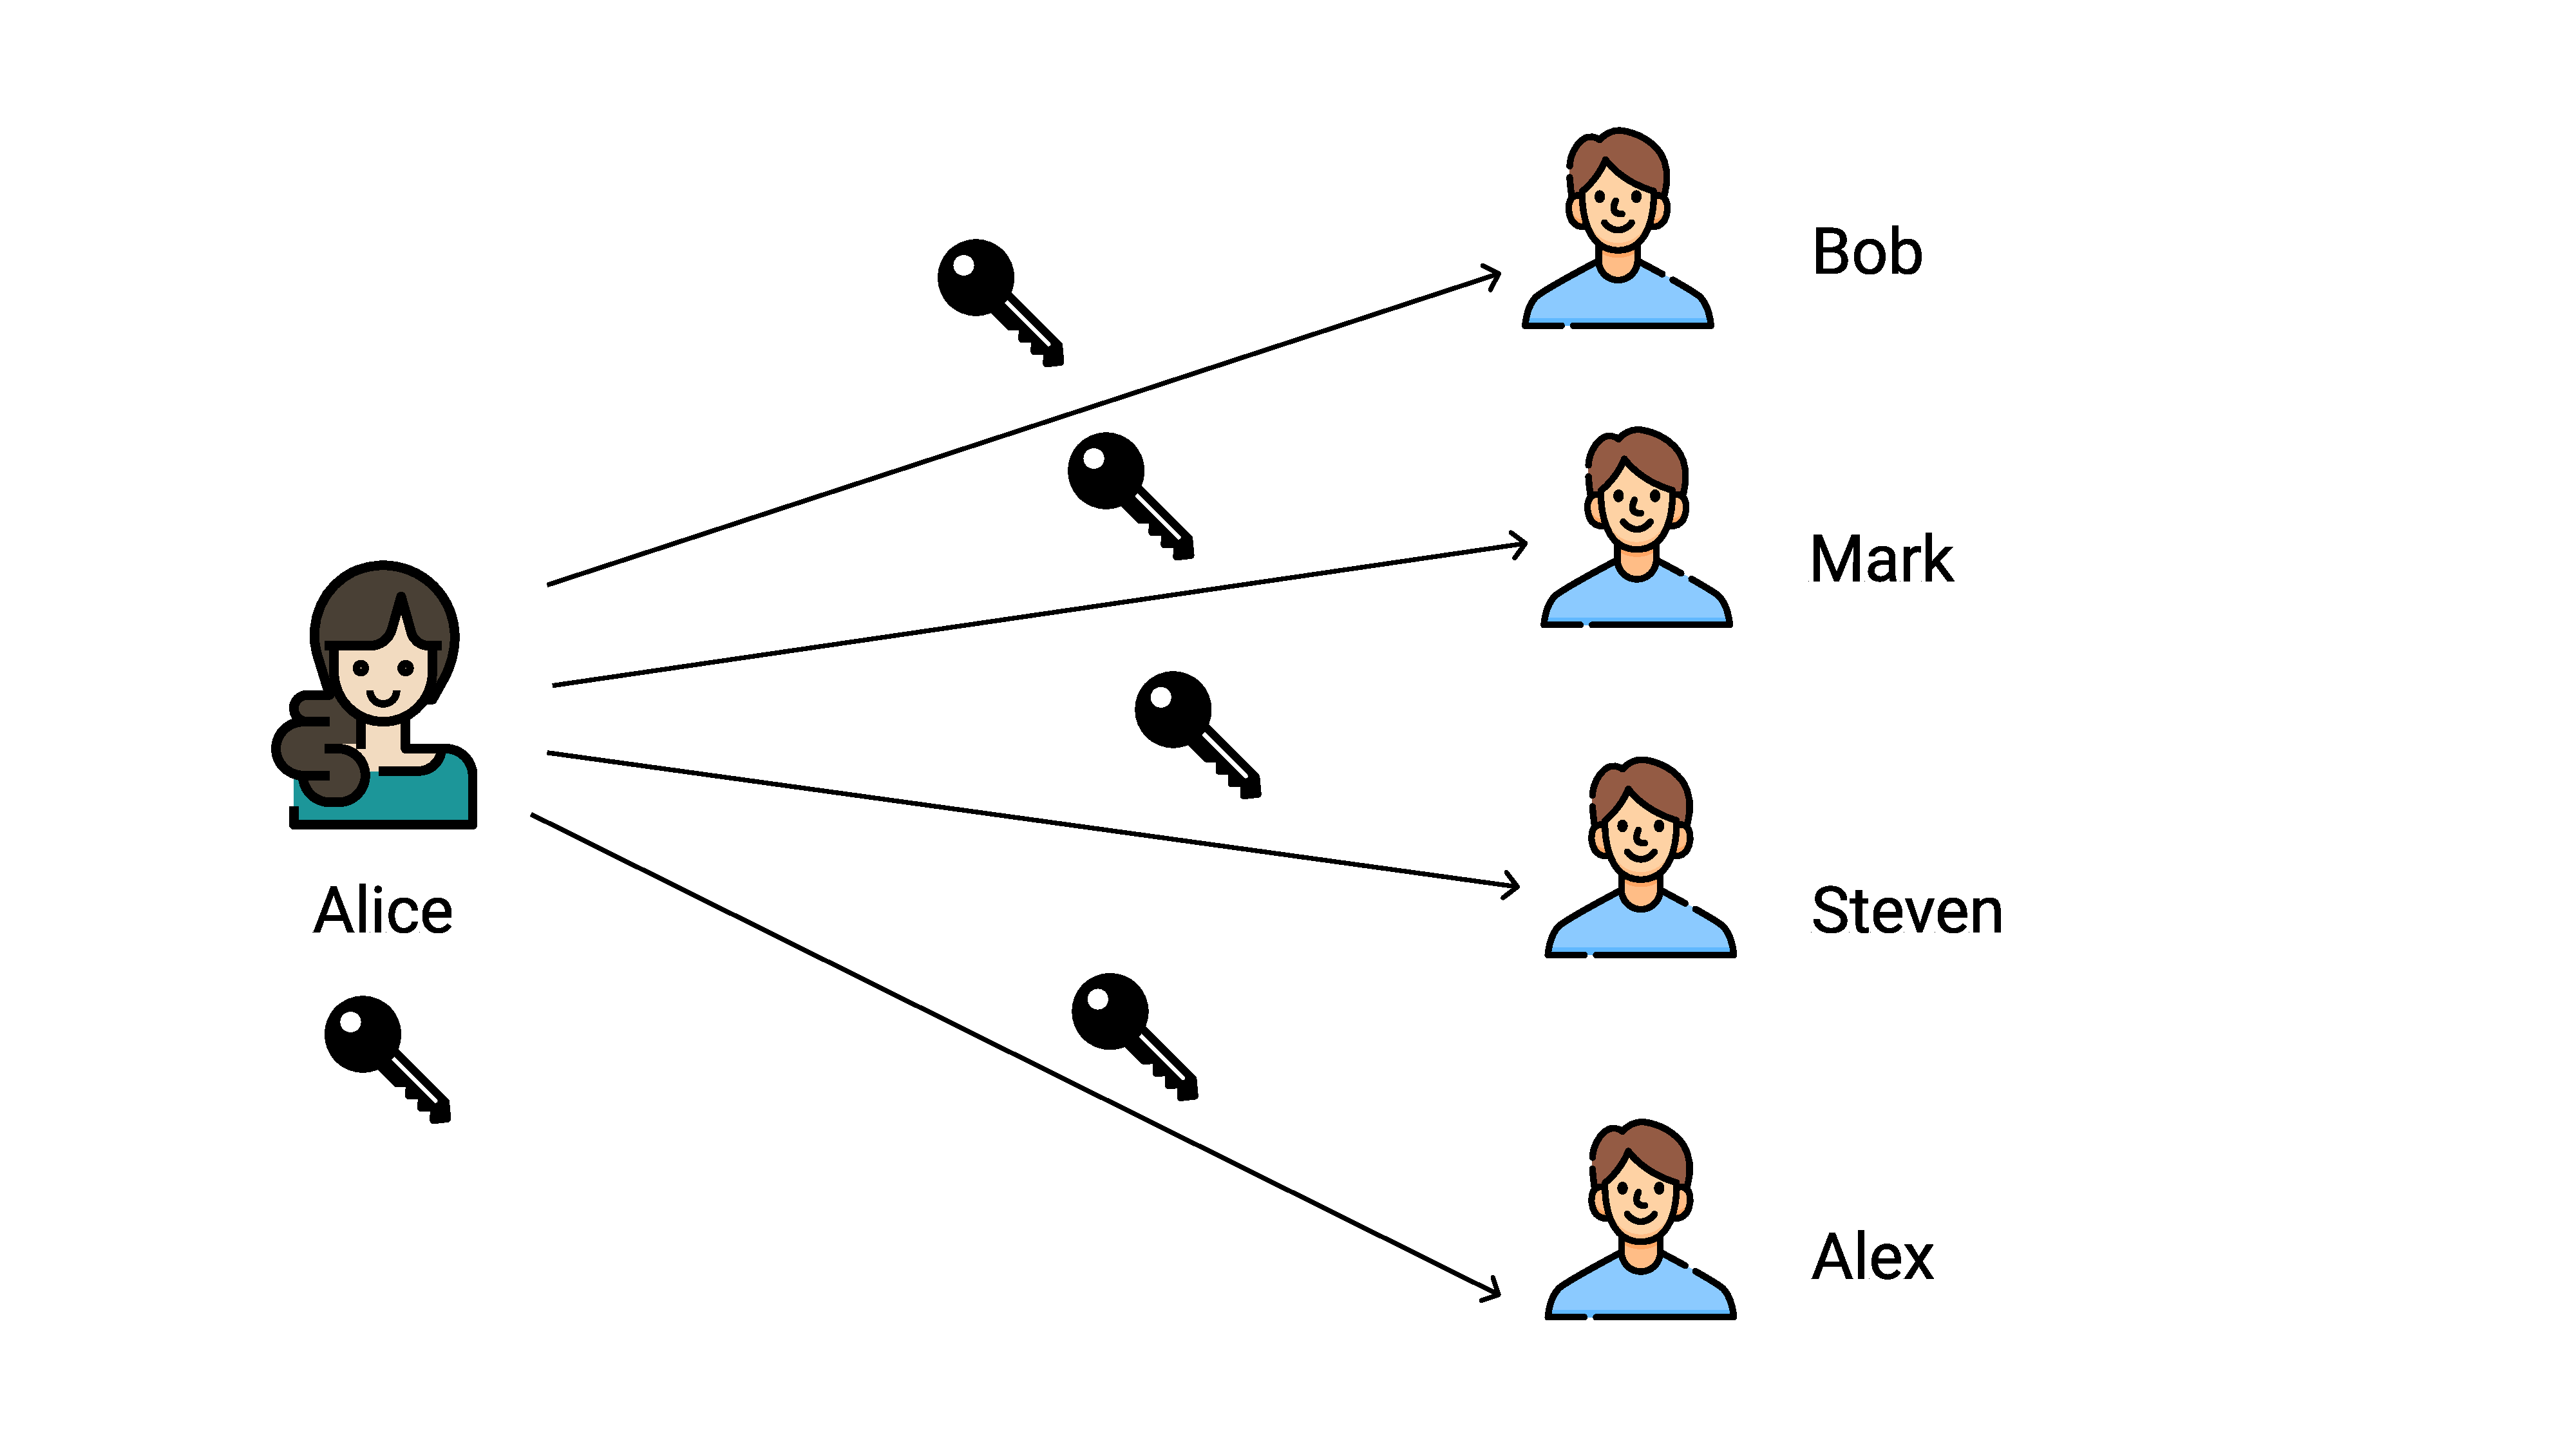
\includegraphics[width=1\textwidth]{Symmetric_encryption}
        ~\caption{Symmetric encryption real life example.}\label{fig:figure}
    \end{figure}

    The problem here is that Alice and Bob must exchange the keys securely, for instance by means of DH key exchange.

    Much more simpler is to think about secured communication channel that in terms of asymmetric encryption.
    \begin{quote}
        \textbf{Asymmetric encryption} -- is an encryption such that a message is encrypted using public key and
        decrypted using private key.
    \end{quote}
    The real life example would be if Alice shares with all the actors not the secret key, but opened lock.
    Still Alice keeps the key with herself, but now she doesn't worry that anyone would lose it so that key exchange must be repeated.
    \begin{figure}[H]
        \centering
        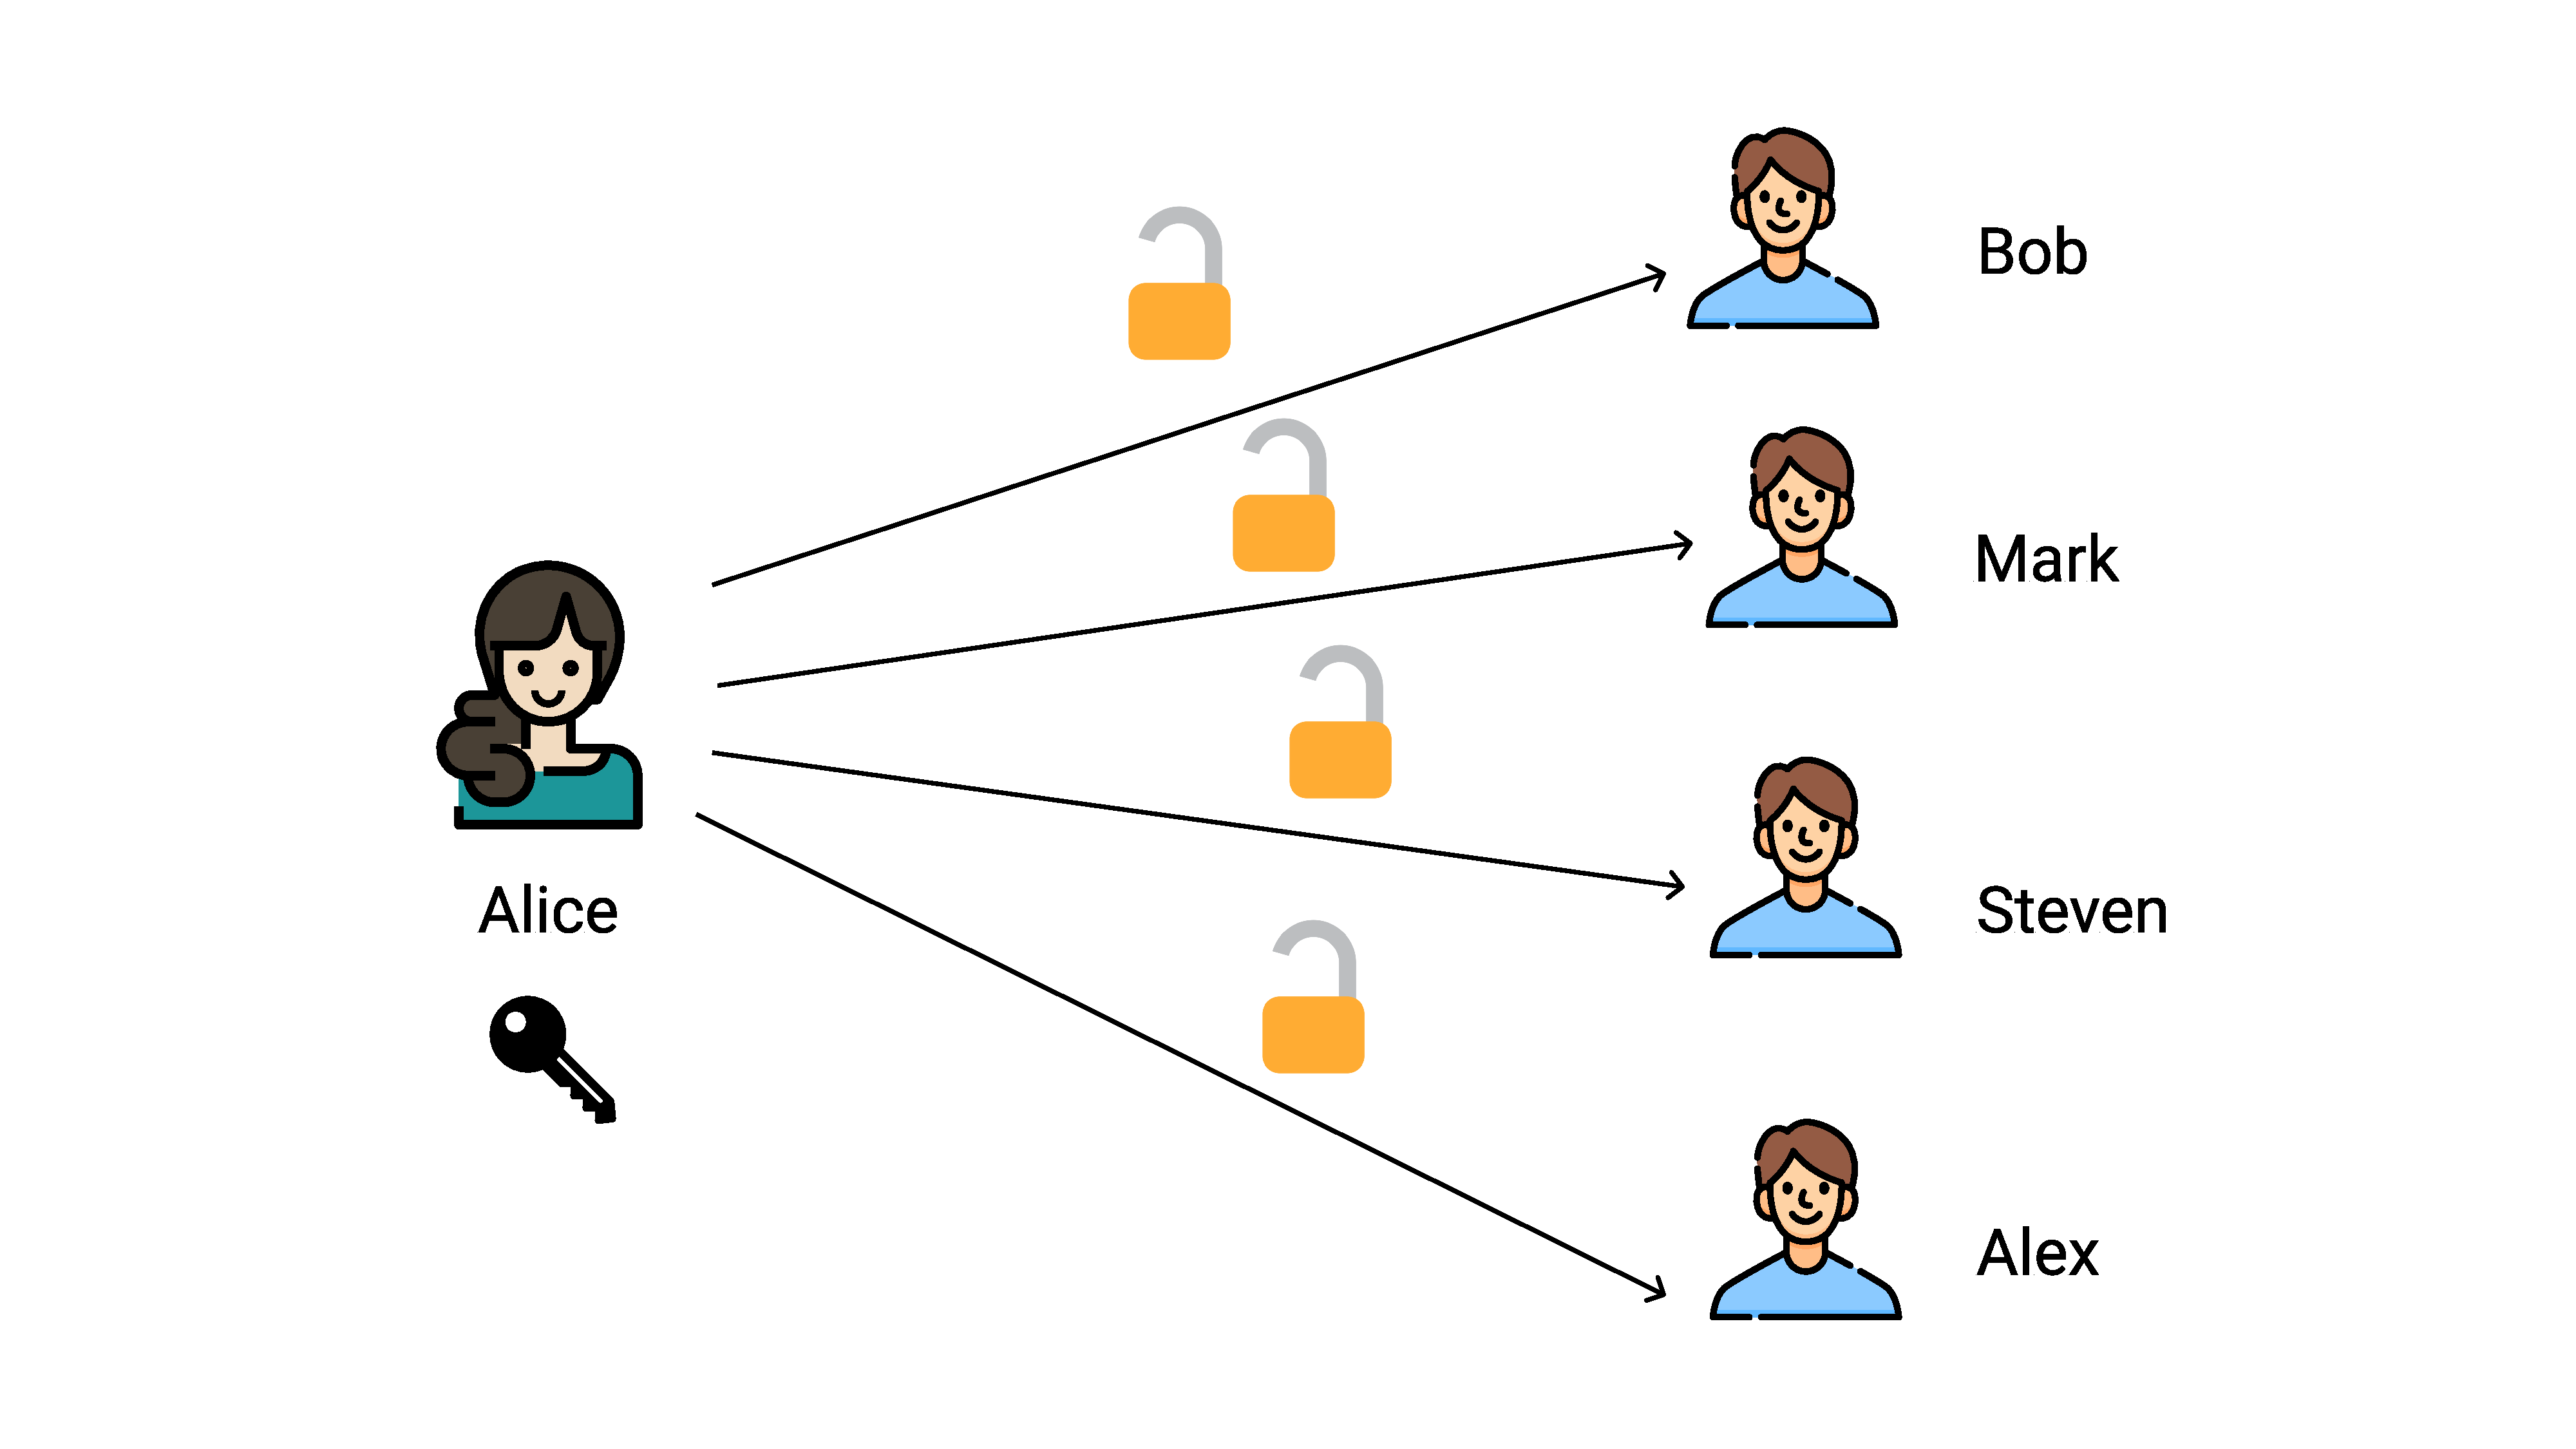
\includegraphics[width=1\textwidth]{Asymmetric_encryption}
        ~\caption{Asymmetric encryption real life example.}\label{fig:figure2}
    \end{figure}
    So that the Bob, Mark, Steven and Alex have received an opened lock from Alice.
    Now anyone of them is able to write secret message to the Alice simply putting it to the chest closing by the lock
    received from Alice so that only Alice can open it.
    However, such a simple idea requires complex number theory approach.
    A concept of opened lock may be interpreted in terms of one-way functions.
    \begin{quote}
        \textbf{One-way function} -- is a function that is easy to compute on every input, but hard to invert given the image of
        a random input.
    \end{quote}


    \section{Mathematics behind RSA}\label{sec:mathematics-behind-rsa}
    For instance, the function
    \begin{equation*}
        f(m) = m^e \bmod N = C, \quad (e, N) \mathrm{\; are \; public \; constants}, \quad m \; \mathrm{is \; secret}
    \end{equation*}
    is one-awy function because it is easy to compute $C$ given $m$, but it is hard to compute $m$ given $C$.
    The constants $(e, N)$ may be interpreted as an Alice's opened lock, whereas $m$ is a secret message from Bob.
    Note that constants
    \begin{itemize}
        \item $e$ is stands for encryption, public key
        \item $d$ is stands for decryption, private key
    \end{itemize}
    Now only one problem remains for the Alice -- is to define a pair of the keys $(e, d)$.
    So, assume that Alice defines two positive integer constants: $e$ is exponent and $N = P \cdot Q$ is public key.
    Alice sends the pair of $(e, N)$ to the Bob so that Bob is able to encrypt his secret message.
    Bob encrypts the secret message $m$ using the one-way function $f(m) = m^e \bmod N$.
    Then Bob sends encrypted message $C$ back to the Alice.
    Given $C$ Alice must fetch the Bob's message $m$.
    In order to decrypt $C$, Alice has to compute
    \[
        C^d \bmod N = m^{ed} \bmod N \equiv m,
    \]
    where $e$ for encryption and $d$ for decryption.
    Now the problem is to define such $d$ that it is hard to the listener to fetch it.
    In order to define the secret $d$, Alice chooses two enough big prime numbers: $P, \; Q$, let's say around 150 digits
    both.
    Then Alice multiplies these two prime numbers in order to get $N$
    \[
        N = P \cdot Q
    \]
    The $N$ is around 300 digits.
    Now Alice can share $N$ with anyone, since it takes decades to find its prime factorization by the fundamental problem
    of prime factorization.
    Next, it is very important to know such a function, which depends on the knowledge of factorization of $N$.
    Such function is an Euler's totient function.
    Given a number $N$ and its prime factorization $p_1^{e_1}\cdot p_2^{e_2} \cdots p_k^{e_k}$, the Euler's totient function
    $\phi(N)$ is defined as
    \[
        \phi(N) = (p_1^{e_1} - p_1^{e_1 - 1}) \cdot (p_2^{e_2} - p_2^{e_2 - 1}) \cdots (p_k^{e_k} - p_k^{e_k - 1})
    \]
    In particular, for positive number $M$ such that its factorization is $p1 \cdot p2$, the $\phi(M)$ is
    \[
        \phi(M) = (p_1 -1) \cdot (p_2 - 1)
    \]
    Euler's theorem relates the modular division and exponent as follows, given number $m$, then
    \[
        m^{\phi(N)} = 1 \bmod N
    \]
    It means that reminder of division $m^{\phi(N)}$ by $N$ is always 1.
    By the equality $1^K = 1$
    \[
        M^{K \cdot \phi(N)} = 1 \bmod N
    \]
    If we multiply both parts by $M$, we get
    \[
        M \cdot M^{K \cdot \phi(N)} = M^{K \cdot \phi(N) + 1} = M \bmod N
    \]
    It follows that Alice is able to define the secret $d$ as follows
    \begin{gather*}
        e \cdot d = K \cdot \phi(N) + 1\\
        d = \frac{K \cdot \phi(N) + 1}{e}\\
    \end{gather*}
    The following image demonstrates the concept of RSA approach
    \begin{figure}[H]
        \centering
        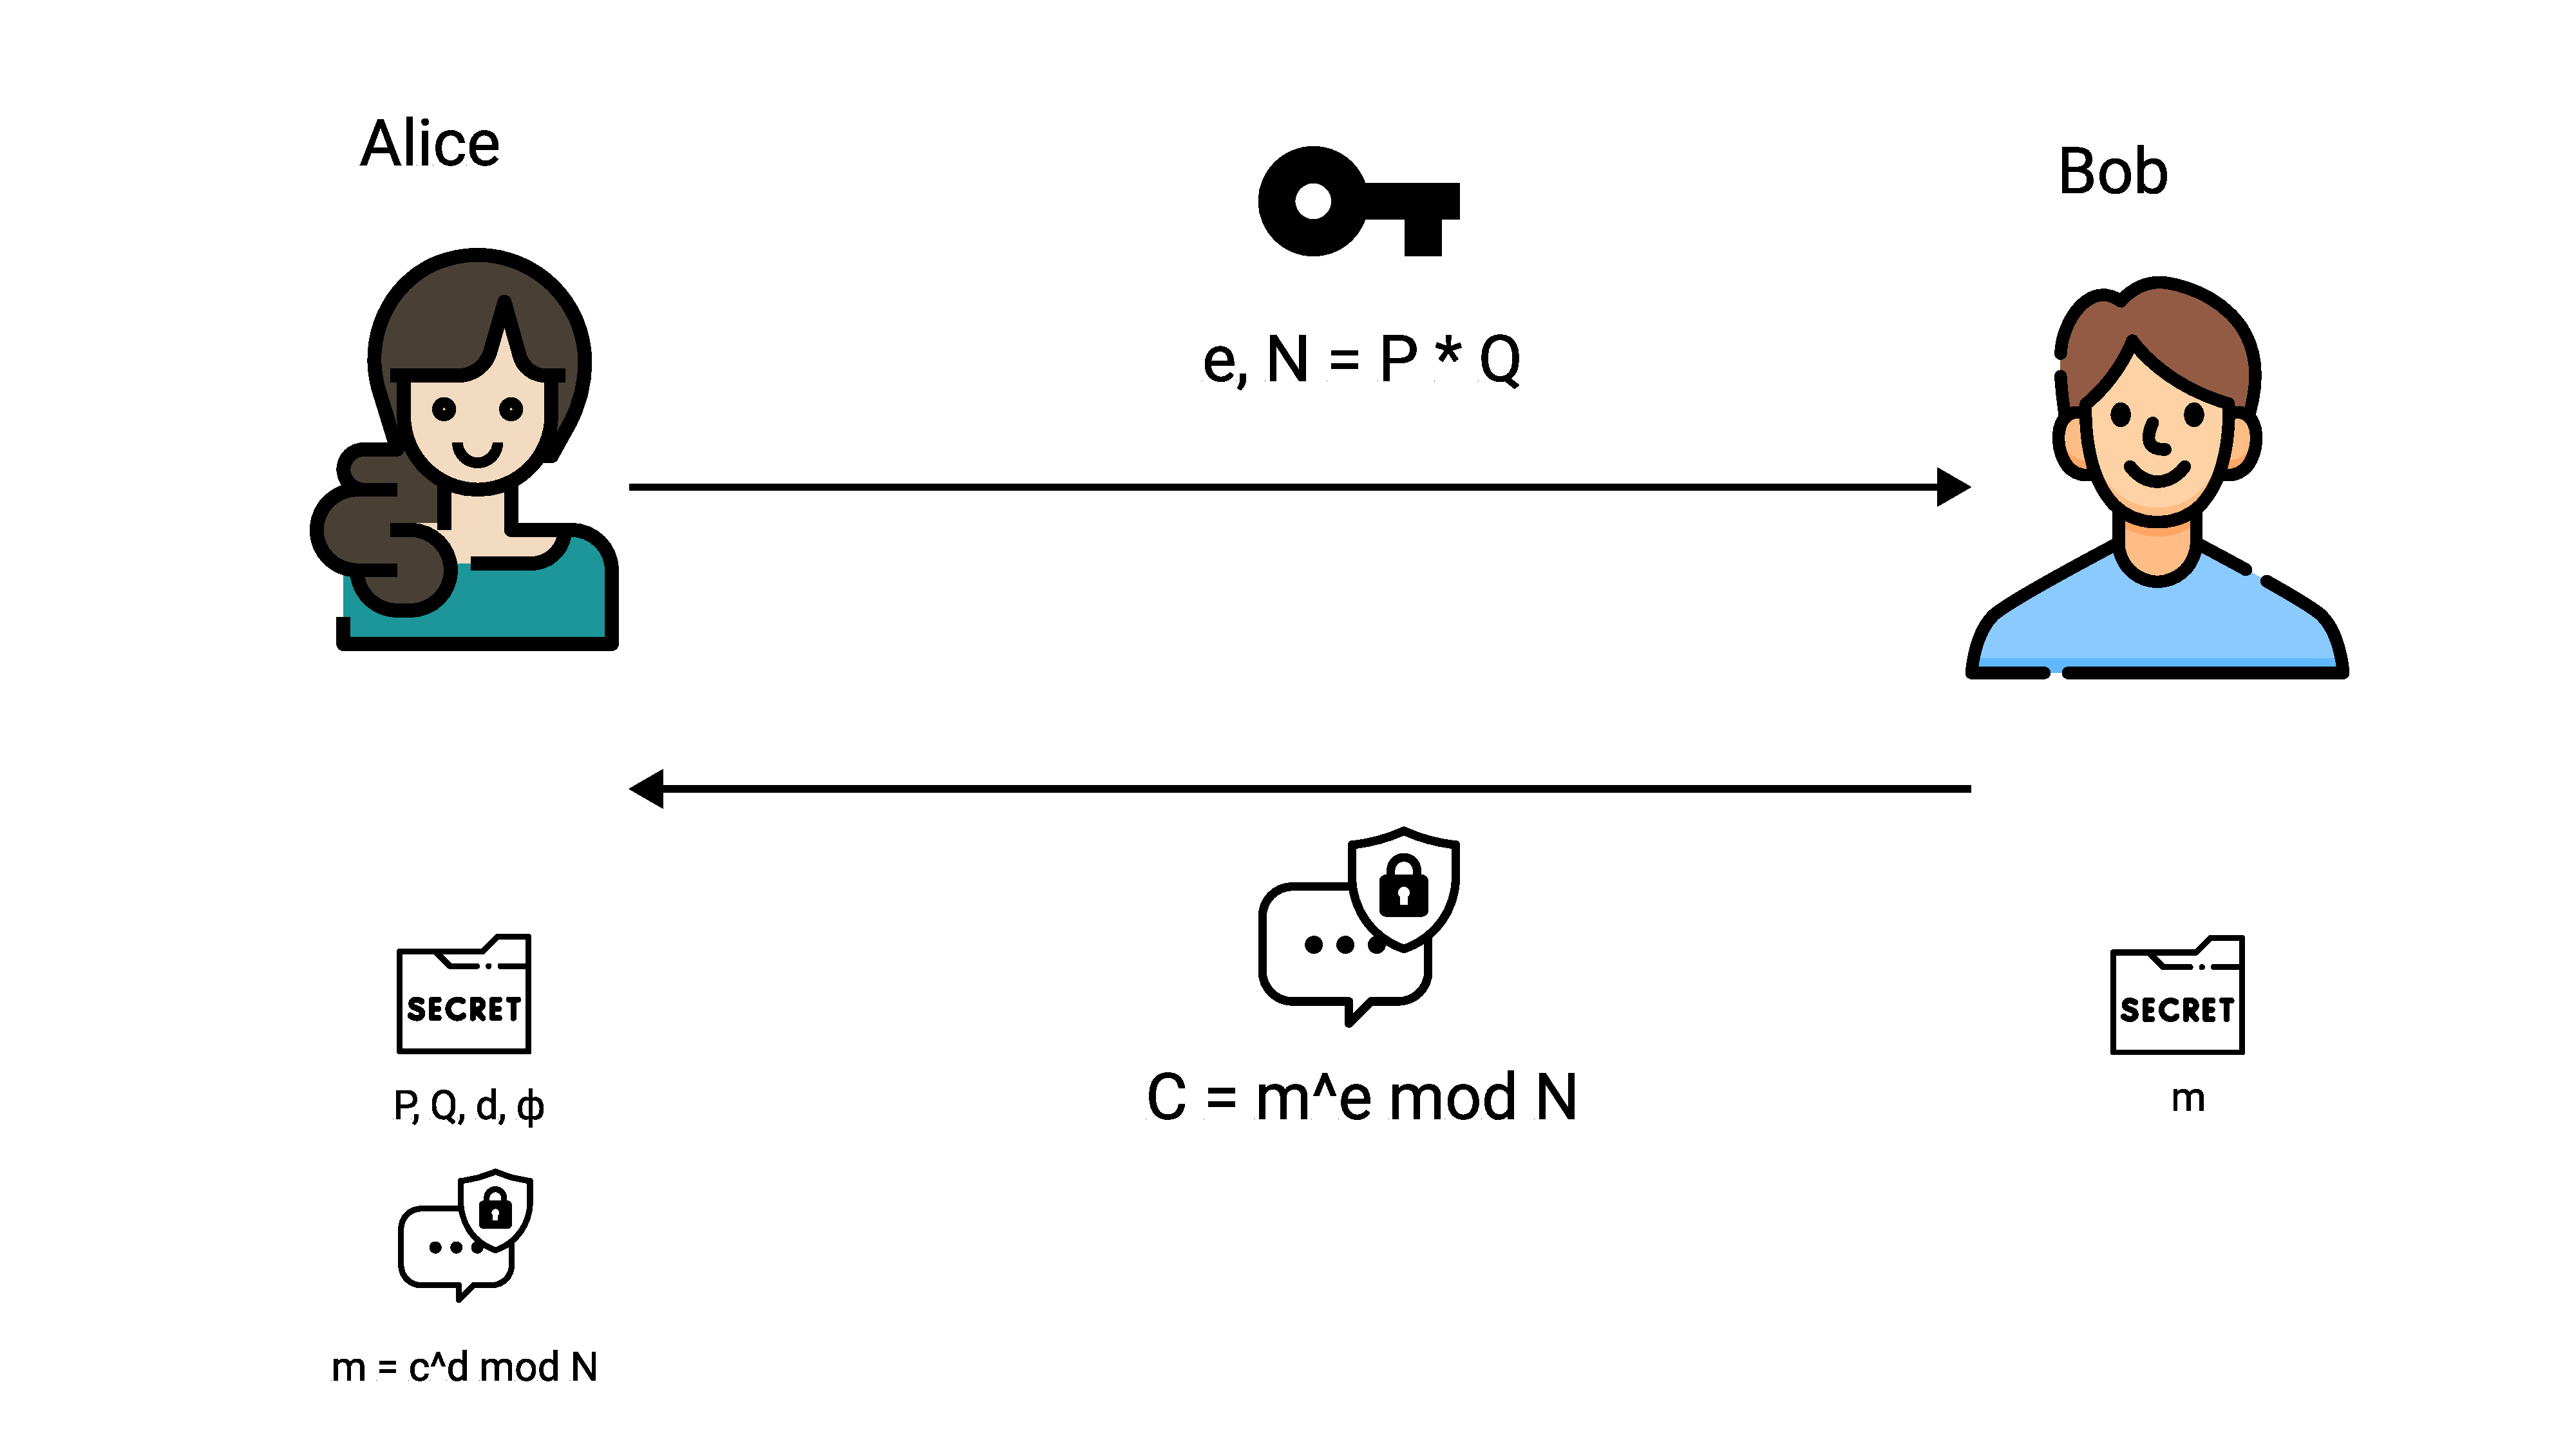
\includegraphics[width=1\textwidth]{12_RSA_encryption_concept_diagram}
        ~\caption{RSA algorithm concept diagram.}\label{fig:figure8}
    \end{figure}
    To summarize, the process by the steps is as follows
    \begin{itemize}
        \item Alice defines the large secret prime numbers $P, \; Q$.
        \item Alice computes $N = P \cdot Q$ and $\phi = (P-1)(Q-1)$
        \item Alice chooses an integer $e$, $1<e< \phi$ such that $\gcd(e, \phi) = 1$.
        \item Alice computes secret exponent $d$, $1<d< \phi$ such that $ed \equiv 1 \bmod \phi$.
        \item Alice shares public key $(N,e)$ with Bob and keeps private key $(d, p, q)$ is secret.
        \item Bob defines the message $m$, encrypts it as $C = m^{e} \bmod N$.
        \item Bob sends $C$ to Alice.
        \item Alice decrypts $C$ using her secret $d$, so she gets $m$
        \[
            m = C^d \bmod N
        \]
    \end{itemize}
    Security of the RSA approach is based on the complexity of fundamental problem of prime factorization,
    which takes decades to solve having enough large number.

    \bibliographystyle{unsrt}
    \bibliography{RSAEncryptionExplained_refs}
\end{document}